% !TeX program = pdflatex
\documentclass[12pt,a4paper]{article}

% --- Pacotes Básicos ---
\usepackage[utf8]{inputenc}
\usepackage[T1]{fontenc}
\usepackage{lmodern}
\usepackage[brazil]{babel}
\usepackage{graphicx}
\usepackage{geometry}
\usepackage{titling}
\usepackage{setspace}
\usepackage{fancyhdr}
\usepackage{amsmath}
\usepackage{siunitx}
\usepackage{url}
\usepackage{indentfirst}
\usepackage{float}
\usepackage{placeins}
\usepackage{caption}
\usepackage{booktabs}
\usepackage{multirow}
\usepackage{hyperref}
\usepackage{xcolor}
\usepackage{tcolorbox}
\usepackage{tabularx}
\usepackage{tikz}
\usepackage{enumitem}

% --- Configurações da página e do rodapé ---
\geometry{
    a4paper,
    top=2.4cm,
    bottom=3.0cm,
    left=2.3cm,
    right=2.3cm,
    headheight=15pt,
    footskip=1.35cm
}
\setstretch{1.35}

\pagestyle{fancy}
\fancyhf{}
\renewcommand{\headrulewidth}{0pt}
\renewcommand{\footrulewidth}{0.8pt}

\fancyfoot[L]{%
    \begin{tabular}{@{}c@{\hspace{0.35cm}}l@{}}
        \raisebox{-0.42\height}{
\includegraphics[height=0.95cm]{images/logo.png}} &
        \begin{tabular}[c]{@{}l@{}}
            \footnotesize\textbf{Instituto Federal de Minas Gerais (IFMG) -- Campus Betim} \\[-2pt]
            \scriptsize Documentação HIL: Simulador Dinâmico (PC + G29 + ESP32 + Speeduino)
        \end{tabular}
    \end{tabular}%
}
\fancyfoot[R]{\footnotesize\textbf{Pág.\ \thepage}}

\setlength{\parindent}{1.25cm}
\setlength{\parskip}{4pt}

\hypersetup{
    colorlinks=true,
    linkcolor=blue!70!black,
    urlcolor=blue!70!black,
    pdftitle={Projeto de Simulacao Dinamica HIL - IF Betim Racing},
    pdfauthor={William Las-Cazas Queiroz}
}

% --- Título ---
\pretitle{%
  \begin{center}
  
\includegraphics[width=4.8cm]{images/logo.png} \\
  \vspace*{0.8cm}
  \LARGE\bfseries
}
\posttitle{\par\vspace{1.2cm}\end{center}}
\preauthor{%
  \begin{center}
  \large
  \lineskip 0.5em%
}
\postauthor{\end{center}}
\predate{\begin{center}\large}
\postdate{\end{center}}

\title{Projeto de Simulação Dinâmica HIL (Hardware-in-the-Loop) \\ \large Interface Serial PC--G29, ESP32 DevKit V1 e ECU Speeduino 48-Way}
\author{
    \textbf{Instituição:} \\
    Instituto Federal de Minas Gerais -- Campus Betim \\[0.8em]
    \textbf{Autor:} \\
    William Las-Cazas Queiroz (0104566) \\
    Gerente Técnico -- Equipe Elétrica \\[0.8em]
    \textbf{Aplicação:} \\
    Validação Dinâmica de Calibração HIL em Malha Fechada (KTM Duke 390)
}
\date{\today}

\begin{document}

\maketitle
\thispagestyle{empty}
\newpage

\tableofcontents
\newpage

% ==========================================
% SEÇÃO 1: INTRODUÇÃO E REPOSITÓRIOS
% ==========================================
\section{Introdução ao Simulador HIL e Recursos do Projeto}

Este documento descreve a arquitetura e o guia completo de reprodução da bancada de simulação dinâmica orientada ao condutor (\textit{Hardware-in-the-Loop} -- HIL) desenvolvida para validação e calibração da ECU \textbf{Speeduino 48-Way}. Na arquitetura adotada, um Computador (PC) atua como \textit{host} USB para leitura em tempo real de um conjunto de volante, pedais e câmbio \textbf{Logitech G29} através de uma interface gráfica em Python/Tkinter, transmitindo os comandos do piloto e os parâmetros físicos do veículo via comunicação Serial (UART) para o microcontrolador da bancada.

O núcleo da planta física é executado em um \textbf{ESP32 DevKit V1 (30 pinos)}, responsável por resolver numericamente a dinâmica longitudinal e rotacional da motocicleta \textbf{KTM Duke 390} ($\sim 373\text{ cm}^3$, monocilíndrica, roda fônica 22-2) e converter as grandezas virtuais em sinais elétricos analógicos e digitais que excitam a ECU em tempo real. A malha de simulação é fechada interceptando os pulsos de injeção e ignição gerados pela Speeduino por meio de interrupções de hardware (ISR).

\begin{tcolorbox}[colback=blue!4, colframe=blue!65!black, title=\textbf{Repositórios Oficiais para Reprodução (Código-Fonte e Mapa Base)}]
Todo o código-fonte do firmware do ESP32, a interface gráfica em Python, o arquivo JSON de parametrização da motocicleta e o mapa base completo da ECU estão disponíveis publicamente nos endereços abaixo:
\begin{itemize}[leftmargin=1.2em, itemsep=4pt]
    \item \textbf{Repositório GitHub (Firmware ESP32, Interface Tkinter e Parâmetros):} \\
    \url{https://github.com/LasCazas/SimulacaoHil.git}
    \item \textbf{Mapa Base da ECU e Configurações do TunerStudio (Google Drive):} \\
    \href{https://drive.google.com/drive/folders/1bbK6THQXaumvtmB5yQu2AqLAyRcFz2Z0}{Clique aqui para acessar a pasta do Mapa Base no Google Drive} \\
    {\footnotesize (\url{https://drive.google.com/drive/folders/1bbK6THQXaumvtmB5yQu2AqLAyRcFz2Z0})}
\end{itemize}
\vspace{2pt}
\footnotesize\textit{Importante:} O arquivo \texttt{.msq} hospedado no Google Drive já contém toda a configuração base da Speeduino 48-Way (decodificador de roda fônica 22-2, mapeamento de portas, calibração de sensores e tabelas iniciais de VE e ignição).
\end{tcolorbox}

% ==========================================
% SEÇÃO 2: LISTA DE MATERIAIS (BOM)
% ==========================================
\section{Lista de Materiais (BOM de Bancada)}

Para montar e reproduzir o ambiente HIL em bancada sem a necessidade de motor ou atuadores indutivos reais, utilizam-se os seguintes itens:

\begin{itemize}[itemsep=3pt]
    \item \textbf{1x Computador (PC) + Conjunto Logitech G29:} Executa a interface gráfica (\texttt{interface\_g29.py}), lê volante, pedais (acelerador, freio, embreagem) e câmbio H/borboletas via USB e comunica-se com o ESP32 a $115200\text{ bps}$.
    \item \textbf{1x Placa ESP32 DevKit V1 (Clássico -- 30 pinos):} Executa a integração numérica da física do motor e do veículo, gera sinais analógicos/PWM/I2S e mede os pulsos de retorno da ECU.
    \item \textbf{1x Módulo DAC de Áudio I2S PCM5102A:} Dedicado exclusivamente à síntese senoidal contínua via DMA da roda fônica \textbf{22-2} (\textit{Crank}) sem sobrecarregar a CPU principal.
    \item \textbf{1x Módulo Conversor de Nível Lógico Bidirecional (2 ou 4 canais -- MOSFET BSS138):} Responsável por condicionar e converter com segurança as saídas lógicas de injeção e ignição da Speeduino para o nível de $3{,}3\text{ V}$ do ESP32 em bancada (sem bobina ou bico físico).
    \item \textbf{2x Filtros Passa-Baixas RC ($R = 10\text{ k}\Omega$, $C = 1\,\mu\text{F}$):} Conectados às saídas nativas de 8 bits \texttt{DAC1} e \texttt{DAC2} do ESP32 ($f_c \approx 15{,}9\text{ Hz}$) para suavizar os degraus de tensão de TPS e MAP antes da leitura pelo ADC da ECU.
    \item \textbf{1x ECU Speeduino 48-Way + Fonte $12\text{ V}$ de Bancada:} Controlador sob teste alimentado pelo pino pós-chave (\texttt{B\_A1}) e referenciado ao mesmo barramento de \texttt{GND} lógico.
\end{itemize}

% ==========================================
% SEÇÃO 3: ARQUITETURA E MODELO MATEMÁTICO
% ==========================================
\section{Arquitetura Lógica e Modelagem Dinâmica}

O simulador opera em três subsistemas acoplados em tempo real:

\begin{enumerate}[itemsep=3pt]
    \item \textbf{Interface Humana (PC + G29):} Aquisita os eixos dos pedais e botões de marcha (1ª a 6ª, Neutro e Ré virtual de bancada), transmite os comandos a $30\text{ Hz}$ para o ESP32 e exibe a telemetria retornada a $20\text{ Hz}$. Também envia dinamicamente pela Serial todos os parâmetros físicos do arquivo \texttt{moto\_duke390.json}, dispensando regravação do firmware ao ajustar a planta.
    \item \textbf{Planta Física Virtual (ESP32):} Integra as equações diferenciais do conjunto motor--embreagem--transmissão--veículo com passo interno de $0{,}5\text{ ms}$:
    \begin{itemize}[itemsep=2pt]
        \item \textbf{Dinâmica do Virabrequim:} A aceleração angular $\dot{\omega}_e$ resulta do balanço na inércia do motor $J_e$:
        \begin{equation}
            J_e \frac{d\omega_e}{dt} = \tau_{\text{ind}}(\omega_e, \text{MAP}, \eta_\lambda) + \tau_{\text{lenta}} - \tau_{\text{atrito}}(\omega_e) - \tau_{\text{emb}}
        \end{equation}
        onde $\tau_{\text{ind}}$ interpola a curva de torque a plena carga (WOT, pico de $\sim 35\text{ N}\cdot\text{m}$ a $7000\text{ RPM}$) modulada pela pressão do coletor (\texttt{MAP}), com limitador de rotação em $10500\text{ RPM}$ e controle proporcional de marcha lenta ($\sim 1400\text{ RPM}$).
        \item \textbf{Acoplamento de Embreagem e Câmbio:} O torque transmitido $\tau_{\text{emb}}$ varia progressivamente conforme o curso do pedal de embreagem e o escorregamento entre $\omega_e$ e a rotação refletida da roda através da redução primária ($2{,}90$), relação da marcha engatada e redução final ($3{,}00$).
        \item \textbf{Dinâmica Longitudinal e Sinal VSS Realista:} A velocidade linear $v$ do veículo é integrada sobre a massa efetiva (moto + piloto + inércia das rodas), descontando arrasto aerodinâmico ($\frac{1}{2}\rho C_d A v^2$), resistência ao rolamento ($C_{rr} m g$) e força de frenagem do pedal de freio. Dessa forma, o sinal \textbf{VSS} é derivado diretamente da rotação da roda: ao pisar na embreagem ou engatar o Neutro em movimento, a frequência do VSS decai suavemente pela inércia do veículo, reproduzindo fielmente o comportamento real em pista.
    \end{itemize}
    \item \textbf{Controlador (Speeduino) e Malha Fechada:} A ECU lê os sensores simulados e comanda injeção e ignição. Quando a chave \texttt{use\_inj\_feedback} está ativa no JSON, o ESP32 compara a largura de pulso real medida no bico (\texttt{INJ-1-OUT}) com a massa estequiométrica admitida por ciclo, escalando a eficiência $\eta_\lambda$ do torque gerado (simulando perda de torque por mistura pobre/rica ou corte de combustível).
\end{enumerate}

% ==========================================
% SEÇÃO 4: MAPEAMENTO DE PINOS E LEVEL CONVERTER
% ==========================================
\section{Mapeamento do Chicote e Condicionamento de Sinais}

Para manter os dois conversores analógicos internos de 8 bits do ESP32 (\texttt{GPIO 25} e \texttt{GPIO 26}) dedicados aos sinais de \textbf{TPS} e \textbf{MAP}, os sinais de relógio do barramento \textbf{I2S} do módulo PCM5102A foram alocados nos pinos \textbf{GPIO 27 (\texttt{BCK})}, \textbf{GPIO 14 (\texttt{LCK/WS})} e \textbf{GPIO 22 (\texttt{DIN})}. A Tabela~\ref{tab:pinout} resume todas as conexões elétricas da bancada.

\begin{table}[H]
\centering
\caption{Mapeamento completo entre ESP32 DevKit V1, condicionamento e Speeduino 48-Way.}
\label{tab:pinout}
\footnotesize
\begin{tabularx}{\textwidth}{@{}llllX@{}}
\toprule
\textbf{Sinal} & \textbf{ESP32} & \textbf{Tipo} & \textbf{Conector ECU} & \textbf{Condicionamento / Observação} \\
\midrule
TPS (Borboleta) & GPIO 25 & DAC1 (0--3,3 V) & \texttt{B\_C7 (TPS)} & Filtro RC ($10\text{ k}\Omega + 1\,\mu\text{F}$) p/ GND \\
MAP (Coletor) & GPIO 26 & DAC2 (0--3,3 V) & \texttt{B\_C8 (MAP-EXT)} & Filtro RC ($10\text{ k}\Omega + 1\,\mu\text{F}$) p/ GND \\
Crank 22-2 (BCK) & GPIO 27 & I2S BCK & \multirow{3}{*}{\texttt{B\_B2 (CRANK-IN)}} & Ligado ao pino \texttt{BCK} do PCM5102A \\
Crank 22-2 (LCK) & GPIO 14 & I2S WS/LCK & & Ligado ao pino \texttt{LCK} do PCM5102A \\
Crank 22-2 (DIN) & GPIO 22 & I2S DATA & & Ligado ao pino \texttt{DIN} do PCM5102A$^{*}$ \\
Velocidade (VSS) & GPIO 16 & PWM LEDC & \texttt{B\_A7 (VSS)} & Onda quadrada $3{,}3\text{ V}$ proporcional a $v$ \\
Embreagem & GPIO 15 & Saída Digital & \texttt{B\_B7 (Clutch\_in)} & Nível lógico indicando pedal acionado \\
Feedback Injetor & GPIO 4 & ISR (\texttt{CHANGE}) & \texttt{G\_A1 (INJ-1-OUT)} & Via Conversor de Nível Lógico (\texttt{Chan2}) \\
Feedback Ignição & GPIO 5 & ISR (\texttt{RISING}) & \texttt{G\_B1 (IGN-1-OUT)} & Via Conversor de Nível Lógico (\texttt{Chan1}) \\
Referência GND & GND & Terra Comum & \texttt{B\_A8} / \texttt{B\_B3} & Unificar GND do ESP32, PCM5102A e ECU \\
\bottomrule
\end{tabularx}
\vspace{2pt}
\raggedright{\scriptsize $^{*}$No módulo PCM5102A, manter o pino \texttt{SCK} aterrado ao \texttt{GND}, alimentar \texttt{VIN} em $5\text{ V}$ e conectar a saída de áudio analógica (\texttt{L}) em \texttt{B\_B2} e o terra de áudio em \texttt{B\_B3 (VR1-)}.}
\end{table}

\subsection{Condicionamento de Retorno com Conversor de Nível Lógico (Bancada sem Bobina e sem Bico Físicos)}

Em um motor real, o acionamento direto de um bico injetor solenoide ou do primário de uma bobina gera picos indutivos reversos (\textit{flyback}) de dezenas a centenas de volts, o que obrigaria o uso de optoacopladores rápidos ou circuitos de grampeamento dedicados. Contudo, \textbf{como na bancada de simulação HIL não conectamos um bico injetor nem uma bobina de ignição reais}, não há carga indutiva nem transientes de alta tensão nas saídas da ECU.

Nessas condições de bancada, um \textbf{Módulo Conversor de Nível Lógico Bidirecional} comercial baseado em transistores MOSFET (como o BSS138 com resistores de \textit{pull-up} integrados de $10\text{ k}\Omega$, ilustrado na Figura~\ref{fig:level_converter}) é perfeitamente capaz de realizar toda a interface elétrica de retorno entre a Speeduino e os pinos de $3{,}3\text{ V}$ do ESP32 (que \textbf{não} são tolerantes a $5\text{ V}$ ou $12\text{ V}$):

\begin{figure}[H]
    \centering
    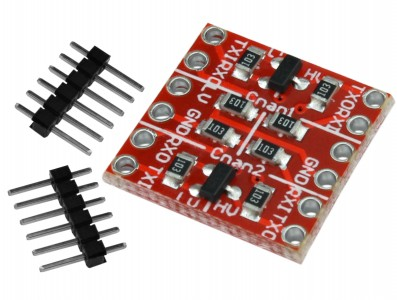
\includegraphics[width=0.42\textwidth]{images/level_Converter.jpg}
    \caption{Módulo Conversor de Nível Lógico Bidirecional de 2 canais (\texttt{HV} $\leftrightarrow$ \texttt{LV}) utilizado para leitura de injeção e ignição sem atuadores indutivos físicos.}
    \label{fig:level_converter}
\end{figure}

\begin{enumerate}[itemsep=4pt]
    \item \textbf{Alimentação de Referência do Módulo:} O pino \textbf{\texttt{HV}} (\textit{High Voltage}) do conversor é alimentado com \textbf{$5\text{ V}$} (fornecidos pelo pino \texttt{5V/VIN} ou fonte lógica da bancada), o pino \textbf{\texttt{LV}} (\textit{Low Voltage}) é conectado ao pino \textbf{$3{,}3\text{ V}$} do ESP32, e os pinos \textbf{\texttt{GND}} de ambos os lados são interligados ao terra comum da ECU.
    \item \textbf{Leitura do Bico Injetor (\texttt{G\_A1 -- INJ-1-OUT} $\rightarrow$ Canal 2 $\rightarrow$ \texttt{GPIO 4}):} A saída de injeção da Speeduino é do tipo \textit{Low-Side} (dreno aberto / \textit{open-drain}): o MOSFET de potência da ECU apenas aterra o pino ao \texttt{GND} durante o pulso de injeção e permanece flutuando quando desligado. Sem o bico físico puxando a linha para $+12\text{ V}$, o resistor de \textit{pull-up} de $10\text{ k}\Omega$ já existente no lado \texttt{HV} do conversor assume o papel de carga fantasma segura (corrente inferior a $0{,}5\text{ mA}$). Em repouso, a linha permanece em nível alto ($3{,}3\text{ V}$ no lado \texttt{LV}); quando a ECU comanda a injeção e aterra \texttt{G\_A1}, o MOSFET do conversor conduz instantaneamente e leva o \texttt{GPIO 4} a $0\text{ V}$, permitindo medir o tempo de injeção em microssegundos.
    \item \textbf{Leitura da Ignição (\texttt{G\_B1 -- IGN-1-OUT} $\rightarrow$ Canal 1 $\rightarrow$ \texttt{GPIO 5}):} Configurada para bobina inteligente (\textit{Smart Coil}), a Speeduino emite pulsos lógicos de $0\text{--}5\text{ V}$. O sinal entra pelo terminal \texttt{HV} do Canal 1 e sai convertido de forma limpa em $0\text{--}3{,}3\text{ V}$ no terminal \texttt{LV} rumo ao \texttt{GPIO 5} do ESP32.
\end{enumerate}

\newpage
% ==========================================
% SEÇÃO 5: DIAGRAMAS VISUAIS
% ==========================================
\section{Diagrama Visual das Conexões Físicas}

\subsection{Envio de Sinais: Conector Preto (B)}
\begin{center}
\vspace*{0.1cm}
\resizebox{0.92\textwidth}{!}{
\begin{tikzpicture}[x=1.1cm, y=1.1cm, >={stealth}]
\tikzstyle{route}=[ultra thick, rounded corners=4pt]
\tikzstyle{lleft}=[left, font=\scriptsize\bfseries]
\tikzstyle{lright}=[right, font=\scriptsize\bfseries]

\filldraw[fill=black!85, draw=black, rounded corners=15pt] (0.2, -1.3) rectangle (8.8, 3.8);
\filldraw[fill=gray!30, draw=black, rounded corners=10pt] (0.4, -1.0) rectangle (8.6, 3.5);

\foreach \x in {1,...,8} {
    \pgfmathsetmacro{\px}{9-\x}
    \node[circle, draw=black, thick, minimum size=0.8cm, inner sep=0pt, fill=yellow!90, font=\scriptsize\bfseries] (A\x) at (\px, 2.5) {B\_A\x};
    \node[circle, draw=black, thick, minimum size=0.8cm, inner sep=0pt, fill=yellow!90, font=\scriptsize\bfseries] (B\x) at (\px, 1.25) {B\_B\x};
    \node[circle, draw=black, thick, minimum size=0.8cm, inner sep=0pt, fill=yellow!90, font=\scriptsize\bfseries] (C\x) at (\px, 0) {B\_C\x};
}

\node[circle, draw=red, line width=2pt, minimum size=1.0cm, inner sep=0pt] at (A1.center) {};
\node[circle, draw=green!70!black, line width=2pt, minimum size=1.0cm, inner sep=0pt] at (A7.center) {};
\node[circle, draw=black, line width=2pt, minimum size=1.0cm, inner sep=0pt] at (A8.center) {};
\node[circle, draw=orange, line width=2pt, minimum size=1.0cm, inner sep=0pt] at (B2.center) {};
\node[circle, draw=orange, line width=2pt, minimum size=1.0cm, inner sep=0pt] at (B3.center) {};
\node[circle, draw=brown, line width=2pt, minimum size=1.0cm, inner sep=0pt] at (B7.center) {};
\node[circle, draw=blue, line width=2pt, minimum size=1.0cm, inner sep=0pt] at (C7.center) {};
\node[circle, draw=purple, line width=2pt, minimum size=1.0cm, inner sep=0pt] at (C8.center) {};

\draw[route, black]          (A8.north) |- (-0.8, 5.0) node[lleft] {\textbf{[GND Comum]} $\rightarrow$ GND (Sensores) - B\_A8};
\draw[route, green!70!black] (A7.north) |- (-0.8, 4.4) node[lleft] {\textbf{[PWM ESP32 GPIO 16]} $\rightarrow$ VSS - B\_A7};
\draw[route, brown]          (B7.north) -- (2, 1.9) -- (1.5, 1.9) |- (-0.8, 5.7) node[lleft] {\textbf{[Digital GPIO 15]} $\rightarrow$ Clutch\_in - B\_B7};
\draw[route, blue]           (C7.south) |- (-0.8, -1.4) node[lleft] {\textbf{[DAC1 GPIO 25 + Filtro RC]} $\rightarrow$ TPS\_Sensor - B\_C7};
\draw[route, purple]         (C8.south) |- (-0.8, -2.1) node[lleft] {\textbf{[DAC2 GPIO 26 + Filtro RC]} $\rightarrow$ MAP-EXT - B\_C8};

\draw[route, red]    (A1.north) |- (9.8, 4.2) node[lright] {B\_A1 - 12V-SW (Pós-Chave) $\leftarrow$ \textbf{FONTE 12V}};
\draw[route, orange] (B2.north) -- (7, 1.9) -- (7.5, 1.9) |- (9.8, 5.5) node[lright] {B\_B2 - CRANK-IN $\leftarrow$ \textbf{PCM5102A (GPIO 27/14/22)}};
\draw[route, orange] (B3.south) -- (6, 0.6) -- (6.5, 0.6) |- (9.8, -2.4) node[lright] {B\_B3 - VR1- $\leftarrow$ \textbf{GND PCM5102A}};
\end{tikzpicture}
}
\end{center}

\subsection{Retorno de Sinais (Feedback): Conector Cinza (G)}
\begin{center}
\vspace*{0.1cm}
\resizebox{0.92\textwidth}{!}{
\begin{tikzpicture}[x=1.1cm, y=1.1cm, >={stealth}]
\tikzstyle{route}=[ultra thick, rounded corners=4pt]
\tikzstyle{lright}=[right, font=\scriptsize\bfseries]

\filldraw[fill=gray!70, draw=black, rounded corners=15pt] (0.2, -1.3) rectangle (8.8, 3.8);
\filldraw[fill=gray!30, draw=black, rounded corners=10pt] (0.4, -1.0) rectangle (8.6, 3.5);

\foreach \x in {1,...,8} {
    \pgfmathsetmacro{\px}{9-\x}
    \node[circle, draw=black, thick, minimum size=0.8cm, inner sep=0pt, fill=yellow!90, font=\scriptsize\bfseries] (A\x) at (\px, 2.5) {G\_A\x};
    \node[circle, draw=black, thick, minimum size=0.8cm, inner sep=0pt, fill=yellow!90, font=\scriptsize\bfseries] (B\x) at (\px, 1.25) {G\_B\x};
    \node[circle, draw=black, thick, minimum size=0.8cm, inner sep=0pt, fill=yellow!90, font=\scriptsize\bfseries] (C\x) at (\px, 0) {G\_C\x};
}

\node[circle, draw=cyan!80!black, line width=2pt, minimum size=1.0cm, inner sep=0pt] at (A1.center) {};
\node[circle, draw=magenta!85!black, line width=2pt, minimum size=1.0cm, inner sep=0pt] at (B1.center) {};

\draw[route, cyan!80!black, ->]    (A1.north) |- (9.6, 4.0) node[lright] {G\_A1 - INJ-1-OUT $\rightarrow$ \textbf{[Level Converter HV$\rightarrow$LV $\rightarrow$ GPIO 4]}};
\draw[route, magenta!85!black, ->] (B1.east) -- (9.6, 1.25) node[lright] {G\_B1 - IGN-1-OUT $\rightarrow$ \textbf{[Level Converter HV$\rightarrow$LV $\rightarrow$ GPIO 5]}};
\end{tikzpicture}
}
\end{center}

% ==========================================
% SEÇÃO 6: SOFTWARE, PROTOCOLO E REPRODUÇÃO
% ==========================================
\section{Estrutura de Software, Protocolo e Guia de Reprodução}

Para manter a documentação enxuta e sempre sincronizada com as evoluções do código, os arquivos executáveis encontram-se organizados no repositório GitHub (\url{https://github.com/LasCazas/SimulacaoHil.git}) conforme abaixo:

\begin{itemize}[itemsep=2pt]
    \item \texttt{HIL\_Esp/HIL\_Esp.ino}: Firmware completo do ESP32 DevKit V1 (compatível com os pacotes Arduino-ESP32 \texttt{2.x} e \texttt{3.x}), integrando síntese DMA I2S da roda fônica 22-2, modelo dinâmico da motocicleta, saídas DAC/PWM e ISRs de injeção/ignição.
    \item \texttt{interface\_g29.py}: Painel gráfico em Python (\texttt{tkinter} + \texttt{pygame} + \texttt{pyserial}) com \textbf{dois modos selecionáveis de operação}: \textit{(i)} \textbf{Modo Volante Real (Logitech G29)}, com barras percentuais e leitura bruta de eixos/botões para calibração; e \textit{(ii)} \textbf{Modo Simulado na Interface (Manual)}, com barras deslizantes (\textit{sliders}) e entradas numéricas de $0\%$ a $100\%$ para os pedais e seletor clicável de marchas (\texttt{R}, \texttt{N}, \texttt{1..6}), permitindo operar e calibrar a ECU na bancada mesmo sem o G29 conectado.
    \item \texttt{moto\_duke390.json}: Arquivo de parametrização documentado contendo 33 parâmetros escalares (inércia, cilindrada, vazão do bico, massa, aerodinâmica, embreagem, sensores), vetor de relações de marcha e curva de torque WOT.
    \item \texttt{config\_g29.json}: Gerado e atualizado automaticamente ao fechar a interface gráfica, salvando a porta COM selecionada, o modo de controle ativo (\texttt{g29} ou \texttt{manual}), o mapeamento de eixos e as inversões dos pedais.
    \item \texttt{CodigoEsp/CodigoEsp.ino}: Código base original de bancada (geração isolada da roda fônica 22-2 via potenciômetros), mantido como referência histórica.
\end{itemize}

\subsection{Protocolo de Comunicação Serial (\texorpdfstring{$115200\text{ bps}$}{115200 bps}, 8N1)}

A troca de mensagens em texto ASCII terminado por quebra de linha (\texttt{\textbackslash n}) segue três formatos:

\begin{table}[H]
\centering
\caption{Mensagens do protocolo Serial entre PC e ESP32.}
\footnotesize
\begin{tabularx}{\textwidth}{@{}llX@{}}
\toprule
\textbf{Direção / Taxa} & \textbf{Formato da Linha ASCII} & \textbf{Descrição dos Campos} \\
\midrule
PC $\rightarrow$ ESP32 ($30\text{ Hz}$) & \texttt{thr,clu,gear,brk\textbackslash n} & \texttt{thr}, \texttt{clu}, \texttt{brk} $\in [0,255]$ (pedais); \texttt{gear} $\in [0,7]$ (\texttt{0}=Neutro, \texttt{1..6}=Marchas, \texttt{7}=Ré). \\
PC $\rightarrow$ ESP32 (Conexão) & \texttt{P,nome,valor\textbackslash n} & Atualiza em RAM qualquer parâmetro do \texttt{moto\_duke390.json} (incluindo \texttt{g1..g6} e pontos \texttt{tqr}/\texttt{tqn}). \\
ESP32 $\rightarrow$ PC ($20\text{ Hz}$) & \texttt{rpm,vss,inj,ign,gr,kmh,tq,map,ff,ok\textbackslash n} & RPM, VSS ($\text{Hz}$), pulso inj.\ ($\mu\text{s}$), idade da centelha ($\text{ms}$), marcha, veloc.\ ($\times 10\text{ km/h}$), torque ($\times 10\text{ N}\cdot\text{m}$), MAP ($\times 10\text{ kPa}$), fator comb.\ ($\times 100$) e status da ECU (\texttt{0/1}). \\
\bottomrule
\end{tabularx}
\end{table}

\subsection{Passo a Passo para Reproduzir o Experimento}

\begin{enumerate}[itemsep=4pt]
    \item \textbf{Configurar a ECU Speeduino no TunerStudio:}
    Baixe o projeto/mapa base (\texttt{.msq}) na pasta do \href{https://drive.google.com/drive/folders/1bbK6THQXaumvtmB5yQu2AqLAyRcFz2Z0}{Google Drive} e carregue-o na Speeduino 48-Way pelo TunerStudio. Como os DACs nativos do ESP32 operam até $3{,}3\text{ V}$ (e não $5{,}0\text{ V}$), realize a calibração de fim de escala do \textbf{TPS} no TunerStudio pisando $0\%$ e $100\%$ no pedal com o ESP32 conectado, e garanta que a faixa do sensor MAP e a vazão de bico coincidam com os valores de \texttt{moto\_duke390.json}.
    \item \textbf{Gravar o Firmware no ESP32 DevKit V1:}
    Abra \texttt{HIL\_Esp/HIL\_Esp.ino} na Arduino IDE (com o pacote oficial \textit{esp32 by Espressif Systems} instalado), selecione a placa \textbf{ESP32 Dev Module} e faça o upload via USB.
    \item \textbf{Montar as Conexões de Bancada:}
    Realize as ligações conforme a Tabela~\ref{tab:pinout} e a Seção~5, certificando-se de instalar os filtros RC nos pinos 25 e 26, aterrar o pino \texttt{SCK} do PCM5102A e alimentar o Conversor de Nível Lógico com \texttt{HV = 5V}, \texttt{LV = 3.3V} e \texttt{GND} comum.
    \item \textbf{Preparar o Ambiente Python e Executar a Interface:}
    Clone o repositório, crie/ative o ambiente virtual e instale as dependências:
    \begin{quote}
    \small\texttt{git clone https://github.com/LasCazas/SimulacaoHil.git}\\
    \texttt{cd SimulacaoHil}\\
    \texttt{python -m venv .venv}\\
    \texttt{.venv\textbackslash Scripts\textbackslash activate}\\
    \texttt{pip install -r requirements.txt}\\
    \texttt{python interface\_g29.py}
    \end{quote}
    \item \textbf{Calibrar o G29 e Operar a Simulação:}
    Com o volante Logitech G29 conectado ao PC (com o Logitech G HUB aberto), selecione a porta \texttt{COM} do ESP32 e clique em \textbf{Conectar}. Após $2\text{ s}$, todos os parâmetros de \texttt{moto\_duke390.json} serão enviados automaticamente. Verifique se cada barra (Volante, Acelerador, Freio e Embreagem) responde ao respectivo pedal — ajustando se necessário o número do eixo ou a caixa \texttt{inv} (suas preferências ficarão salvas automaticamente ao fechar a janela). Para alterar características da moto ou ativar a malha fechada de combustível (\texttt{"use\_inj\_feedback": 1}), basta editar \texttt{moto\_duke390.json} e clicar em \textbf{Reenviar parâmetros}.
\end{enumerate}

\end{document}
